\documentclass[10pt,letterpaper]{article}

\usepackage{cogsci}
\usepackage{pslatex}
\usepackage{graphics}
\usepackage{graphicx}
\usepackage{gensymb} %for symbols such as the degree sign
\usepackage{xcolor}
\usepackage{array}% http://ctan.org/pkg/array
\usepackage{tabularx}
\usepackage{booktabs}% http://ctan.org/pkg/booktabs
\usepackage{multirow} %to have multiple row entries in tables
\usepackage{enumitem} %better environment for lists 
\usepackage{breakurl} %to break urls
\usepackage{amsmath}

\usepackage[natbibapa]{apacite}
\usepackage[font=small]{caption}  %smaller figure captions
\usepackage[compact]{titlesec} %space around section headings
\usepackage[textsize = tiny]{todonotes}
\setlength{\marginparwidth}{1.5cm} %sets the comment margin
%\usepackage[font=scriptsize]{subfig} %for creating panels
%\usepackage[countmax]{subfloat} %for creating panels
%\usepackage{wrapfig} %to wrap figures
%\usepackage{float}  %for floating figures
%\usepackage{hyperref} %to have links within the document
%for possessive citing
\def\citeapos#1{\citeauthor{#1}'s (\citeyear{#1})}

%title spacing 
\titlespacing{\section}{0pt}{*0.5}{*0.5}
\titlespacing{\subsection}{0pt}{*0.5}{*0.5}
\titlespacing{\subsubsection}{0pt}{*0.1}{*1}

%footnote page breaking penalty
\interfootnotelinepenalty=10000

\newcommand{\ttodo}[2][]
{\todo[caption={#2}, size=\small, #1, color = orange, inline]{\renewcommand{\baselinestretch}{1}\selectfont \textbf{TG}: #2}~}

\newcommand{\sttodo}[2][]
{\todo[caption={\textbf{TG}}, size=\footnotesize, color = orange, #1]{#2}~}

\newcommand{\ntodo}[2][]
{\todo[caption={#2}, size=\small, #1, color = yellow, inline]{\renewcommand{\baselinestretch}{1}\selectfont \textbf{NB}: #2}~}

\newcommand{\rtodo}[2][]
{\odo[caption={#2}, size=\small, #1, color = blue, inline]{\renewcommand{\baselinestretch}{1}\selectfont \textbf{RM}: #2}~}

\newcommand{\sntodo}[2][]
{\todo[size=\footnotesize, color = yellow, #1]{#2}~}

\newcommand{\srtodo}[2][]
{\todo[size=\footnotesize, color = green, #1]{#2}~}

\setlength{\marginparwidth}{1.5cm}

\title{Causal learning from interventions and dynamics in continuous time}
 
\author{{\large \textbf{Neil R. Bramley$^1$} (neil.bramley@ucl.ac.uk)}, {\large \textbf{Ralf Mayrhofer$^2$} (rmayrho@gwdg.de)}\\{\large \textbf{Tobias Gerstenberg$^3$} (tger@mit.edu), {\large \textbf{David A. Lagnado$^1$} (d.lagnado@ucl.ac.uk)}}\\
{\small$^1$Department of Experimental Psychology, UCL, London, WC1H 0DS, UK}\\
{\small$^2$Department of Psychology, University of G{\"o}ttingen, Gosslerstr. 14, 37073, Germany}\\
{\small$^3$Department of Brain and Cognitive Sciences, MIT, Cambridge, MA 02139, USA}
}

%\href{mailto:neil.bramley@ucl.ac.uk}{neil.bramley@ucl.ac.uk}),
% Tobias Gerstenberg (\href{mailto:tger@mit.edu}{tger@mit.edu}),
% Ralf Mayrhofer (\href{mailto:rmayrho@gwdg.de}{rmayrho@gwdg.de}),
% David Lagnado (\href{mailto:d.lagnado@ucl.ac.uk}{d.lagnado@ucl.ac.uk})
\graphicspath{
{figures/}
}

%Operators %TODO do we use all these?
\DeclareMathOperator*{\Do}{Do}
\DeclareMathOperator*{\pa}{pa} %Parents

\newcommand{\ww}{\mathbf{w}} %Parameter
\newcommand{\ws}{w_S} %Parameter
\newcommand{\wb}{w_B} %Parameter

\newcommand{\mm}{s} %Single causal model
\newcommand{\mmm}{S} %Random variable causal models
\newcommand{\cald}{\mathcal{D}} %Set of data
\newcommand{\calc}{\mathcal{C}} %Set of interventions
\newcommand{\calm}{S} %Set of models

\newcommand{\ci}{\mathbf{i}} %Single intervention
\newcommand{\ccc}{C} %Set of interventions
\newcommand{\da}{\mathbf{d}} %Data

\DeclareMathOperator*{\zz}{\mathbf{z}} %Actual causation
\DeclareMathOperator*{\zzz}{\mathbf{Z}} %Actual causation

\begin{document}

\maketitle

\begin{abstract}
Event timing and interventions (actions that manipulate causal variables) are important and intertwined cues to causal structure, yet they have typically been studied separately.  We bring them together for the first time in an experiment where participants learn causal structure by performing interventions in continuous time.  We contrast learning in acyclic and cyclic devices, and reliable and unreliable cause--effect delays.  We show that successful learners use their interventions to structure and simplify their interactions with the devices and that we can capture judgment patterns with heuristics based on online construction and testing of a single structural hypothesis.\\
\textbf{Keywords:} 
causal learning; intervention; time; dynamics
\end{abstract}

%\section{Introduction}

In a dynamically unfolding world, using actions to uncover causal relationships requires good timing.  It is hard to tell whether a new medication is effective if you take it with others, or just as you start to feel better.  Likewise, it is hard to tell whether a new law lowers crime if it is introduced just after other reforms or before a major election.  Such inferences, having to do with delayed effects and an evolving causal background, can be particularly tough in cyclic systems in which feedback loops make prediction difficult even with complete knowledge \citep{brehmer1992dynamic}.  Thus, for interventions to be effective tools for unearthing causal structure it is important to time and locate them carefully, paying close attention to the temporal dynamics of surrounding events and the possibility of feedback loops. 

%\ttodo{it would be good to emphasize both the continuous time aspect of the task, as well as the loopiness -- both of which are features that have been neglected in the causal structure learning literature}

Previous work has shown that people make systematic use of temporal information, taking event order as a strong cue to causal order \citep{bramley2014order}, and making stronger attributions when putative cause--effect delays are in line with expectations \citep{buehner2006temporal,hagmayer2002temporal} and have low variance across instances \citep{greville2010temporal}. Recent work has also developed frameworks for probabilistic causal inference from event timings based on parametric assumptions about cause--effect delays \citep{bramley2017time,pacer2015upsetting}.

A distinct line of work has shown that people are adept at inferring causal structure from interventions --- idealized actions that set variables in a system \citep[e.g.,][]{bramley2017neurath,coenen2015strategies}. This work has not explored the role of temporal information however. 
% , although this has focused on scenarios where effects are revealed simultaneously making time uninformative.  
While researchers have speculated about the close relationship between temporal and interventional inference \citep[e.g.,][]{lagnado2004advantage}, our paper is the first to explore interventional causal learning in continuous time. 
% no one has yet studied interventional causal learning in continuous time. 

\section{The learning problem}

We explore the general problem of figuring out how a causal system works by interacting with it in continuous time.
We focus on abstract causal ``devices'' made up of 3--4 components (cf. Figure \ref{fig:examples}).
For causally related components, we assume each activation of a cause will tend to bring about a single subsequent activation of its effect after a parametric delay (described below).  For example, Figure \ref{fig:examples}a shows a learner's interactions with a $B\leftarrow A \rightarrow C$ Fork during which time they perform four interventions.  Activations of both $B$ and $C$ succeed the interventions on $A$ but with some variability in delays.

We focus on situations with no spontaneous component activations, but where causal relationships work stochastically (e.g. are successful with probability $\ws$). Any pair of components can be connected in either, neither or both directions resulting in a hypothesis space $\calm$ of 64 possible structures for devices made up of three components, and 4096 for four components.  Learners can intervene on the devices by directly activating any component at any moment of their choosing. Interventions are always successful in that they instantaneously activate the targeted component. The downstream causal effects of intervened-on components are the same as those of components that were activated by other components. Thus, we model the consequences of interventions in analogy to the $\Do(.)$ operator introduced by \cite{pearl2000causality}, such that interventions provide no information about the causes of the intervened-on component.

\begin{figure}[t]
   \centering
   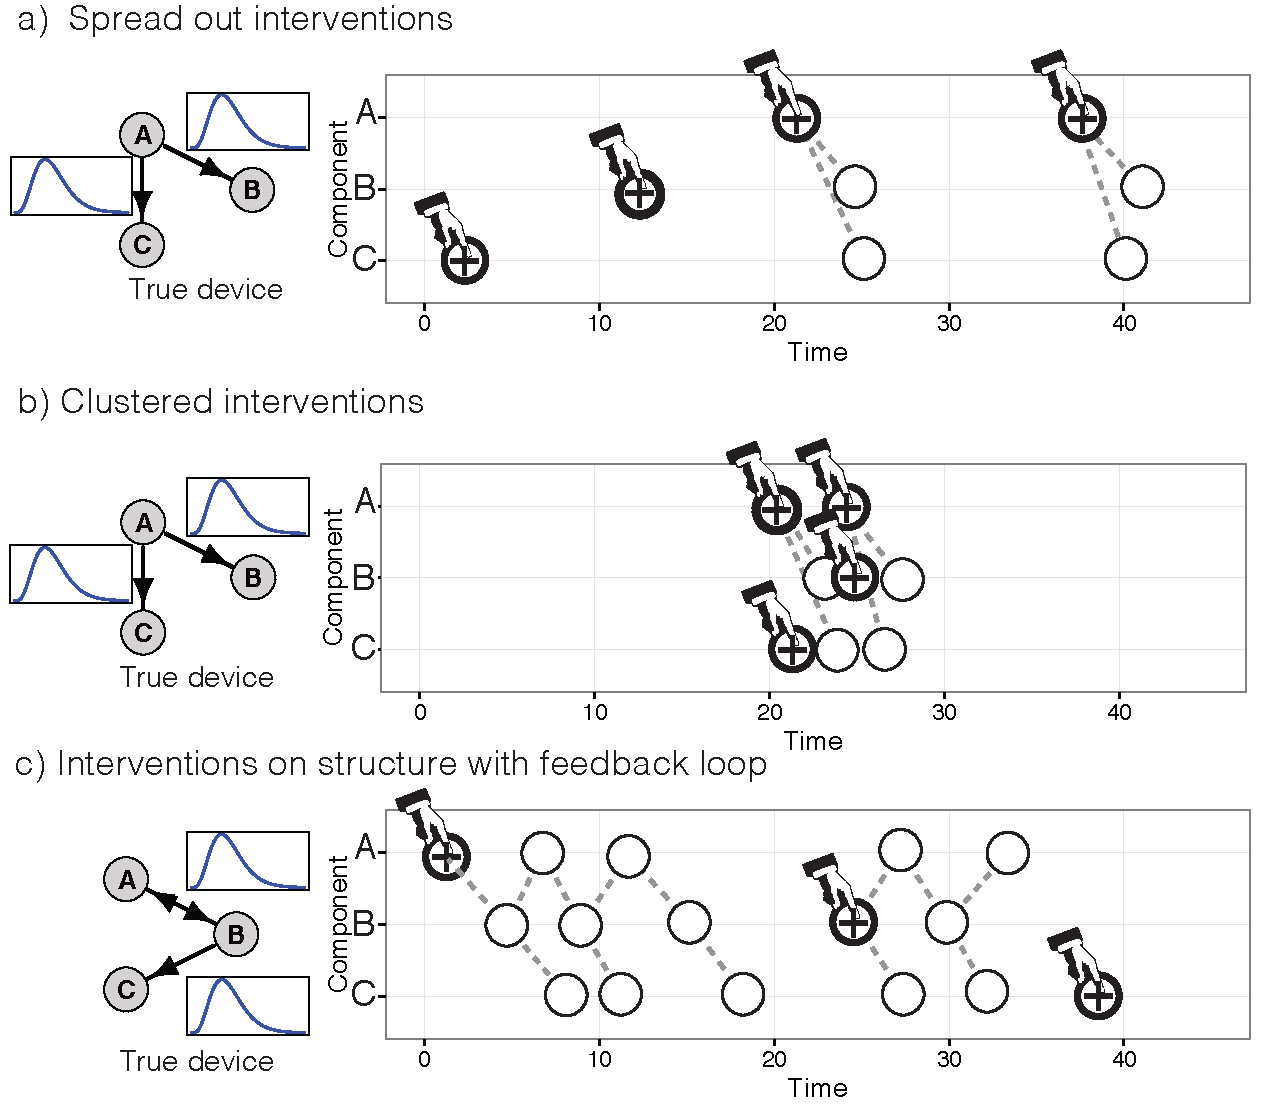
\includegraphics[width = \columnwidth]{examples}
   \caption{Examples of using real-time interventions to infer causal structure. Left: True generative causal model with subplots showing delay distributions. Right: Timelines showing an active learners' interactions with each system with a row for each component and circles indicating component activations.  ``+'' symbol and incoming hand icon indicate interventions.  Dashed gray lines indicate the actual cause--effect relationships.}
   \vspace{-0.6cm}
   \label{fig:examples}
\end{figure}


\subsection{Choosing interventions}

Seeing the effects of one's interventions in continuous time provides rich information for causal inference. On the flip side, there are also no completely independent trials. 
For instance, in Figure~\ref{fig:examples}a, the early interventions on $B$ and $C$ might, in principle, be responsible for the observed effects.  In general, one cannot rule out that something that happened earlier is still exerting its influence, or that an effect is yet to reveal itself.  Fortunately, interventions provide anchor points. We know that events due to interventions weren't caused by anything else, and that these events only affect the future but not the past \citep{lagnado2004advantage}. 
This means that by intervening, learners can recreate some of the advantages that come with a discrete trial structure.  
For example, by waiting long enough between interventions to be confident effects have dissipated, an otherwise confusing event stream becomes more palatable and informative about the underlying structure. 
Figure~\ref{fig:examples}b gives an example of interventions on a $B\leftarrow  A\rightarrow C$ Fork device that are not well chosen.  The learner performs four interventions in the same locations as Figure~\ref{fig:examples}a but does so in close succession. It is hard to attribute causal responsibility for these activations, since there are so many similarly plausible candidates. Consequentially, this data is considerably less informative.

In discrete-trial interventional learning, participants exhibit a \emph{positive testing strategy} --- they prefer to intervene on root variables that bring about many effects \citep{coenen2015strategies}.  While often not leading to the most globally informative choice, a positive testing strategy is an effective way of assessing the adequacy of one's current working hypothesis, making it a manifestation of confirmation biased testing \citep{nickerson1998confirmation}.  Many other components will be affected if one's hypothesis is right, and few if it is wrong.  Repeated positive testing might be more justifiable in the continuous time context because cause--effect delays may play out differently each time, and potential temporal reversals between variable activations will help to rule out candidate structures \citep{bramley2014order}. 
% for instance, allowing learners to rule out structures through order reversals \citep{bramley2014order}. 
For example, in Figure~\ref{fig:examples}a the second intervention on $A$ leads to $B$ and $C$ occurring in reversed order, allowing the learner to rule out a $A\rightarrow B\rightarrow C$ Chain structure.

\subsection{Causal cycles}

The vast majority of causal learning studies have focused on acyclic causal systems in which causal influences flow only in one direction, never revisiting the same component.  However, many natural processes are cyclic and people frequently report cyclic relationships when allowed to do so \citep[e.g.][]{sloman1998feature}.  While there are ways of adapting the causal Bayes net formalism to capture cycles \citep{rehder2016cycles}, these generally simplify the problem to influences between fixed time steps \citep[e.g.][]{rottman2012causal}, or just to the long-run equilibrium distribution \citep[e.g.][]{lauritzen2002chain}.  However, by focusing on continuous time and developing a representation capable of modeling causal dynamics, we are able to directly compare learning in acyclic and cyclic causal systems.%\ttodo{this is a really big deal i think -- we should make clear to sufficiently highlight this in the paper (i.e. make sure to have it in the intro as well as the GD at the end)}

% Not much is known about how people learn in cyclic causal structures. 
%Previous work on cyclic structures has focused on the problem of controlling the system rather than learning its underlying causal structure \citep[e.g.][]{brehmer1992dynamic,osman2011controlling}.  
Dynamic systems can be hard to predict even with perfect knowledge.  Feedback can lead to sensitive dependence on initial conditions with very different behavior resulting from small perturbations in starting conditions \citep[e.g.][]{gleick1997chaos}.  
%Thus, we hypothesize that complex dynamics will support for particular structure hypotheses harder to evaluate, and cyclic causal structures correspondingly harder to learn than acyclic ones.
% , potentially requiring different interventional strategies to manage the complexity.  
Figure~\ref{fig:examples}c gives an example of interventions on a cyclic causal system (assuming that the connections work 90\% of the time).  Interventions initialize looping behavior because of the bidirectional relationship $A \leftrightarrow B$ (e.g., $A\rightarrow B \rightarrow A \rightarrow B\ldots$) leading to many subsequent activations of both the loop components and the output component $C$, continuing until either the $A\rightarrow B$ or $B\rightarrow A$ connection fails. Based on simply looking at the timeline, it seems likely that it will be easier to identify which components are either directly involved in cycles, or outputs from cyclic components (due to their recurrent activations), but harder to identify the exact causal relationships (e.g. whether it is $A$ or $C$ that causes $B$ in this example since both tend to recur shortly before $B$).

%In order to look formally at learning in cyclic and noncylic systems we must develop a normative framework that can handle cases where components can exhibit multiple activations and cause--effect relationships have parametric delays.

\begin{figure*}[t]
   \centering
   \vspace{-.9cm}
   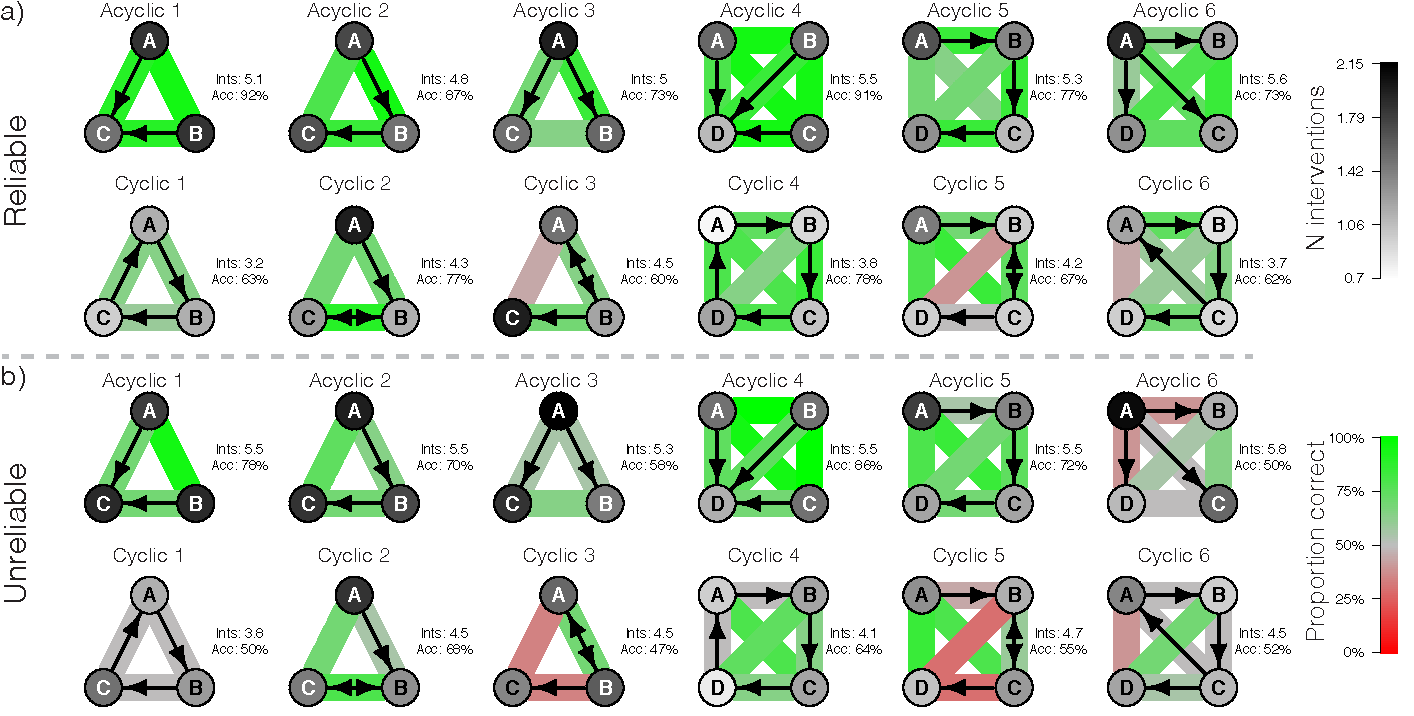
\includegraphics[width = .95\textwidth]{results_cond_numbered}
   \caption{Test models and results from experiment in a) \emph{reliable} and b) \emph{unreliable} delay conditions.  \textbf{Node shading:} Intervention choice prevalence by component.  \textbf{Edge shading:} accuracy.   Average number of interventions performed and accuracy to right of each structure.}
   \label{fig:results_cond}
   % \vspace{-0.6cm}
\end{figure*}

\subsection{Normative inference}
As a benchmark, we developed a Bayesian model of causal structure inference for which we consider the data $\da_{\tau}\left\{ d_X^{(1)},\ldots, d_X^{(n)} \right\}$ to be made up of all activations (with events indexed in chronological order and $X$ indicating the activated component) conditioned upon the set of interventions $\ci_{\tau}=\left\{i_X^{(1)},\ldots, i_X^{(m)} \right\}$ both restricted to the interval between the beginning of the clip and time $\tau$, which we assume to be the moment in which the learner makes the inference.  For instance, one might interact with a causal device for 5000 ms, performing interventions on components $A$ and $B$: $\ci_{5000} = \{i_A^{(1)}=100, i_B^{(2)}=1200\}$, and observing two activations of $C$: $\da_{5000} = \{ d^{(1)}_C=1500, d^{(2)}_C=2800\}$.

Normative Bayesian structure inference involves updating a prior over structure hypotheses $P(\calm)$ with the likelihood $p(\da_{\tau}|\calm;\ci_{\tau}, \ww)$ to get a posterior belief over structures $P(\calm|\da_{\tau};\ci_{\tau}, \ww)$ given the set of parameters $\ww$:\footnote{In this specific case, we assume the parameters (i.e., causal strength $\ws$, expected length of delays $\mu$, and delay variability $\alpha$) to be known which is consistent with the setup of the experiment.}

\begin{equation}
    P(\calm|\da_{\tau};\ci_{\tau}, \ww) \propto p(\da_{\tau}|\calm;\ci_{\tau}, \ww) \cdot P(\calm)
\end{equation}

An immediate issue with calculating the likelihood of an observed set of activations given a candidate model is that there are likely to be multiple potential paths of \emph{actual causation} that could have produced the data \citep{halpern2016causality}, each of which implying a different likelihood.  For example, if the true structure is a $A\rightarrow C \leftarrow B$ Collider, the data above might be produced in two ways.  $A$ could have caused the first activation of $C$ and $B$ the later ($c_A^{(1)}\rightarrow d_C^{(1)}, c_B^{(1)}\rightarrow d_C^{(2)}$).  Alternatively, $A$ could have caused the later activation of $C$ and $B$ the earlier ($c_A^{(1)}\rightarrow d_C^{(2)}, c_B^{(1)}\rightarrow d_C^{(1)}$). 

However, as there can only be one true path of actual causation in the set of possible paths $\zzz_{\mm}$, we can sum over these to get the likelihood of the data given a candidate model $\mm\in\calm$:

\begin{equation}
p(\da_{\tau}|\mm;\ci_{\tau}, \ww) = \sum_{\zz^\prime \in \zzz_{\mm}}p(\da_{\tau}|{\zz}^{\prime}; \ci_{\tau}, \ww)
\label{eq:ti_mar_li}
\end{equation}

We assume that the actual causal delays (in $\zzz_{\mm}$) are Gamma distributed (see also \citealp{bramley2017time}) with a known expected duration $\mu$ and shape $\alpha$ (i.e., variability). The likelihood of the data given a specific path $\zz^\prime$, then, is the product of the (Gamma) likelihoods of the observed delays and causal strength $\ws$ combined with the likelihoods of (non-)events, the occurrence of which failed either due to the $1-\ws$ causal failure rate or due to the effect potentially occurring after $\tau$ (i.e., some time in the future).

With these ingredients, the posterior belief over causal structure hypotheses can be determined. However, it is only feasible to enumerate all possible paths of actual causation for a sufficiently small number of events. While for a large number of events the calculations become intractable, we were able to compute the posteriors in the described manner for the data from the current experiment, resorting only in rare cases to an approximation.\footnote{Where necessary, we ruled out actual causation paths that implied an implausibly large number of failed connections or extreme cause--effect delays, doing so until the number of paths be summed over fell below $100,000$.}


%\subsection{Heuristic inference}

%\subsubsection{Order or timing?}

%\sntodo{Do we need another sentence here?, i.e. that people can be sensitive strong enough delay expectations.  Alternatively could collapse this para in with earlier paragraph on time?}A number of studies have suggested that human causal learning from time is more readily driven by event order than by exact timings \citep{bramley2014order,mccormack2015temporal}.  For example, based on the evidence in Figure~\ref{fig:examples}a, an order-driven learner would (initially) favor an $A\rightarrow B\rightarrow C$ Chain after observing $B$ then $C$ activate, since this is line with the order they observed the events even though the intervals are more consistent with $C$'s being caused by $A$.

%\subsubsection{Model discrimination or construction?}

%For complex structure learning, the range of possible structures, interventions and outcomes quickly becomes unmanageable.  Therefore, several papers have proposed human causal learning is based in the adaptation of a single global hypothesis \citep{bonawitz2014win}, which might be achieved incrementally through making local changes as data is observed \citep{bramley2017neurath}. This seems particularly applicable in a continuous-time context, where normative inference is tough and the evidence, by its nature, arrives continuously.  
%One idea is that people learn locally, ignoring dependence on beliefs about surrounding relationships \citep[e.g.][]{fernbach2009causal}.  Another is that learners use their current model as a basis, comparing observations against the predictions of their model, only adding new connections to explain events that cannot easily be accommodated by the existing model \citep{bramley2017neurath}.  We explore these possibilities in modeling participants' judgments later in the paper.

%Past proposals along these lines have differed in the extent to which participants' updated judgments are shaped by their current beliefs (refs).  In terms of diagnosing the causes of effects, lots of basic work has suggested shorter intervals, but \citep{buehner2006temporal,greville2010temporal,bramley2017time} suggest greater sensitivity. \ttodo{i didn't get the last sentence}

%With more than a few components, the number of possible structures $|M|$ becomes enormous, making storage and computation of $p(M)$ infeasible.  Thus, to explain human ability to learn complex causal structure, a number of papers have proposed that human structure learning is based in the adaptation of a single global hypothesis \citep{bonawitz2014win}, which might be achieved incrementally through making local changes as data is observed \citep{bramley2017neurath}.  Thus learners might construct their causal models ``locally'' by attributing effects to preceding events as they occur, for instance adding new connections to their model when it is unable to accommodate some newly observed effect.   



\section{Experiment}

Participants' task was to discover the causal connections between the components of several devices in limited time (see Figure~\ref{fig:results_cond}). Half of the devices were \emph{acyclic} (top; no feedback loops) and half were \emph{cyclic} (bottom; contained a feedback loop).
Participants were able to activate any of the components by clicking on them. 
We were interested in how participants chose \emph{where} to intervene and \emph{when}.  We examined two delay conditions between subjects, one in which the true cause--effect delays were \emph{reliable} (Gamma distributed with $\alpha=200, M\pm SD~1.5\pm0.1$ seconds) and one where they were \emph{unreliable} ($\alpha=5, M\pm SD~1.5\pm0.7$ seconds). 
Following \cite{greville2010temporal}, we expected that performance would be better when causal delays were \emph{reliable}.  We also predicted complex dynamics would lead to worse performance when the true structure was \emph{cyclic}, and successful participants would spread their interventions widely over time, thus minimizing the ambiguity of resulting patterns of effects.

\subsection{Methods}

\subsubsection*{Participants}
 
Forty participants (14 female, aged $32\pm 9.0$) were recruited from Amazon Mechanical Turk (yielding 20 subjects in each delay-reliability condition) and were paid between \$0.50 and \$3.20 (\$$2.06\pm0.39$) depending on performance (see Methods section).  The task took around 20 minutes.

\begin{figure*}[t]
%\vspace{-1cm}
%$\vspace{0.2cm}
   \centering
   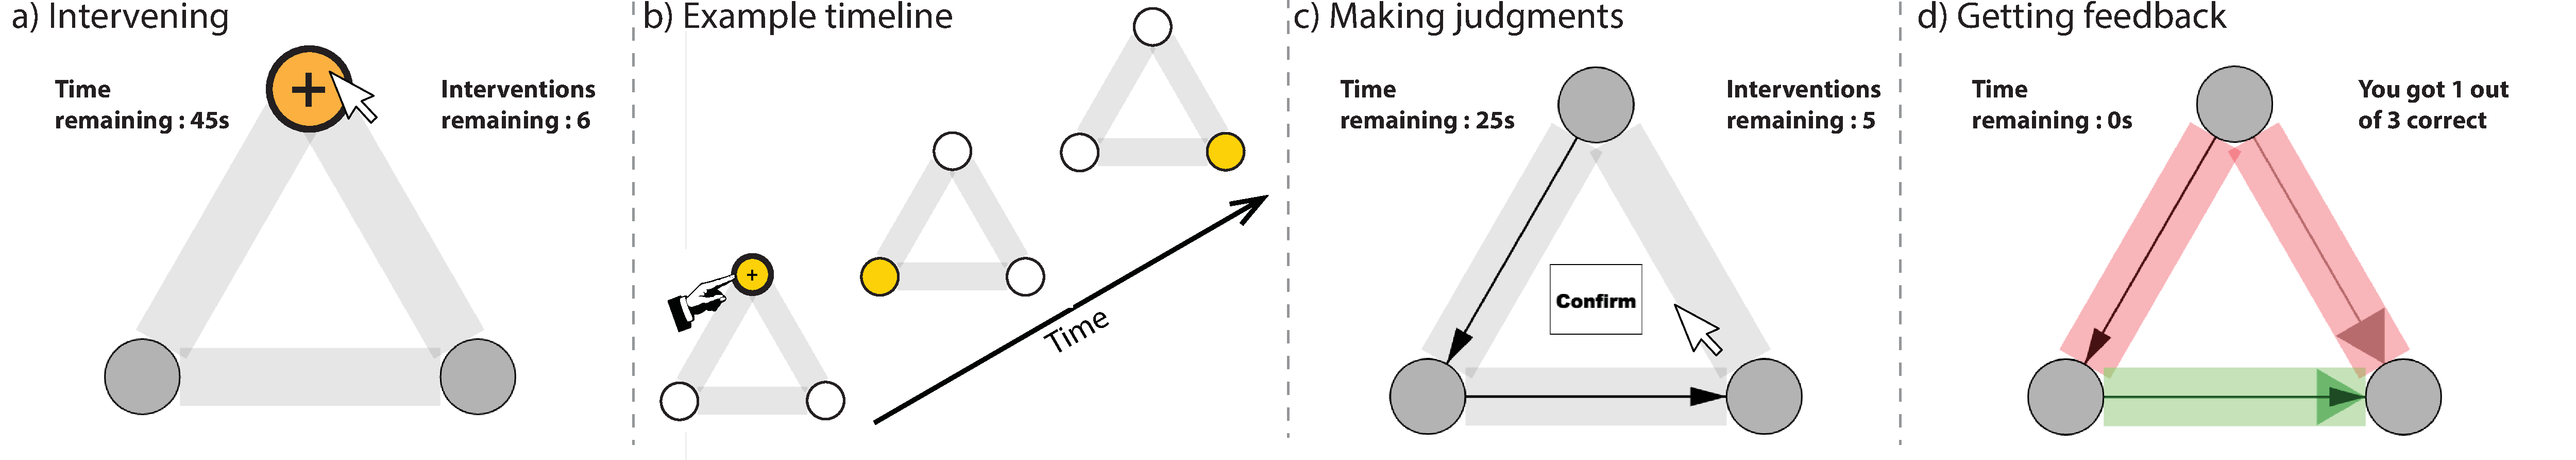
\includegraphics[width = .98\textwidth]{procedure}
   \caption[Experimental procedure]{Experimental procedure. a) Up to 6 interventions could be performed by clicking on the components during the 45 second trial.  b) This would lead to subsequent activations determined by causal connections and delays in the true model.  c) Participants marked their beliefs about the structure during the trials by clicking on the edges.  d) At the end of each trial they received feedback.}
   \label{fig:procedure}
   \vspace{-0.6cm}
\end{figure*}

\subsubsection*{Materials and procedure}

%The task was programmed in javascript, hosted online, 

Each device was represented with a circle for each component and boxes marking the locations of the potential connections (see Figure~\ref{fig:procedure}a).\footnote{Try the task \url{https://www.ucl.ac.uk/lagnado-lab/el/it} or watch a trial \url{https://www.ucl.ac.uk/lagnado-lab/el/itv}.} 
Trials lasted for 45 seconds during which components activated if clicked on or if caused by the activation of another component, with delay and probability governed by the true underlying network (Figure~\ref{fig:procedure}b).  Causal relationships worked 90\% of the time (i.e., causal strength $\ws=0.9$) and there were no spontaneous activations.  Activated components turned yellow for 200ms, and intervened-on components were additionally marked by a ``+'' symbol. Initially, all components were inactive and no connections were marked between them.

Prior to the inference tasks, participants were trained on the delays in their condition and how to register structure judgments through interaction with an an example device.  They then had to correctly answer comprehension check questions and complete a practice problem, before facing the 12 test devices in random order with randomly orientated and unlabeled components.

In the test phase, participants could perform up to 6 interventions on each trial and register/update their judgments about the causal structure as often as they liked until the 45 seconds for a device ran out (for details see Figure~\ref{fig:procedure}). At the end of each trial, they were given feedback showing the true relationships and which of them they had correctly identified. To incentivize proper judgments, bonuses were paid based on connections participants had registered at a randomly chosen point during each trial. 



\subsection{Results}
We analyze participants' judgments by first comparing their accuracy by delay-reliability condition (between subjects: \emph{reliable} vs. \emph{unreliable}) and device type (within subject: \emph{acyclic} vs. \emph{cyclic}).  We then analyze the timing and spacing of participants' interventions and how these relate to the evidence and judgments.


\subsubsection{Accuracy}

Participants updated and confirmed their judgment about the structure $1.6\pm1.2$ times per trial on average.  Judgment time was not significantly related to accuracy, but within trials, final judgments were slightly more accurate than initial judgments, with participants correctly identifying $69\%\pm30$\% compared to $65\%\pm28$\% of the connections, $t(479) = 5.2, p<.001$ (recalling that random bonus times incentivised making judgments early where possible; chance was 25\%). %\ttodo{what did you do in situations in which participants only made one judgment at the very end? if participants make judgments earlier, this could just mean that they focused on one link -- so they might be right about that, but don't have a less good score overall (i.e. building up their structure as they go along)). what's the motivation for making judgments earlier in the first place?}  
Only 4\% of judgment updates decreased the number of connections, 24\% resulting in the same number as before, and 72\% increasing the number of connections.

Focusing on final judgments, participants correctly identified [\emph{reliable,acyclic}]: $82\%\pm29\%$,  [\emph{reliable,cyclic}]: $68\%\pm28\%$,  [\emph{unreliable,cyclic}]: $69\%\pm29\%$,  [\emph{unreliable,cyclic}]: $56\%\pm29\%$ of the connections (see Figure~\ref{fig:results_cond}).  A repeated measures analysis revealed a significant effect of delay-reliability condition, $F(1, 38)=4.6, p<.001$, and cyclicity, $F(1, 38)= 39, p<.001$, but no interaction, with \emph{unreliable} delays and \emph{cyclic} structures associated with lower accuracy.  This figure shows that participants found the Cyclic 3 and Cyclic 5 structures hardest to identify on average, struggling in particular with distinguishing looping from output components.


Ideal Bayesian inference based on the evidence generated by participants predicts a different pattern.  While \emph{reliable} delays allow greater accuracy than \emph{unreliable} ones, $F(1,38) = 24.3, p<.001$, there is no predicted difference in accuracy between \emph{acyclic} and \emph{cyclic} devices, $F(1, 38)= 0.43, p=.5$.  In fact, posterior uncertainty over all possible models, measured by Shannon entropy, was generally lower for evidence generated by a \emph{cyclic} $.74\pm1.26$ than an \emph{acyclic} $1.95\pm1.29$ devices, $F(1,38) = 109, p<.001$.%, and participants accuracy by trial is anticorrelated with an ideal learner's $r=-.45$.

\subsubsection{Timing of interventions}

We hypothesized that spacing interventions out in time would be important for successful learning.  Participants waited $7.3\pm2.8$ seconds between interventions on average.  In a regression including delay condition and total number of interventions as covariates, leaving longer intervals between interventions was positively associated with accuracy, $F(1,36)=14.0, \beta = 0.04, \eta^2_p=.26, p=.001$, with no interaction with condition.  The variability of these gaps --- measured by their coefficient of variation $CV = \frac{\sigma}{\mu}$ --- was also inversely related to accuracy, $F(1,36)=7.9, \beta = -0.5, \eta^2_p=.18, p=.008$ and this effect was stronger in the \emph{unreliable} delay condition, $F(1,35) = 4.5, \eta^2_p=.11, p=.04$.  We also assessed the intervals participants left after the most recently preceding event (whether this was an intervention or an effect) before performing their next intervention.  Again larger intervals, $F(1,36)=7.7, \beta = 0.06, \eta^2_p=.18, p=.008$, and less variation, $\beta=-.25, F(1,36)=5.0, \eta^2_p=.12, p=.03$, was associated with accuracy with neither measure interacting with delay condition. 
Both larger intervals between interventions, and between interventions and the most recently preceding effect were also associated with lower posterior entropy, with $\beta=0.05, F(1,36)=9.9, \eta^2_p=.22, p=0.003$ and $\beta=0.09, F(1,36)=8.1, \eta^2_p=.18, p=0.007$, respectively.  However, there was no relationship between entropy and the variability of either interval type.

\subsubsection{Positive testing}
We found evidence of a preference for positive testing, with participants performing $1.2\pm0.5$ times as many interventions per root component than per non-root component $t(59) = 3.9, p<.001$. 
This preference was associated with higher accuracy after accounting for condition, $F(1,37) = 21, \eta^2_p = 0.37, p<.001$, and did not interact with condition.  Degree of root preference, however, had no affect on posterior uncertainty from the perspective of an ideal Bayesian learner.

\subsubsection{Adaptation to cycles}

While participants performed fewer interventions on  \emph{cyclic} ($4.1\pm1.1$) compared to \emph{acyclic} ($5.4\pm0.7$) devices, $t(39) = 8.7, p <.001$ (see Figure~\ref{fig:results_cond}), they still experienced far more effects in the \emph{cyclic} systems ($29.3\pm10$) compared to the \emph{acyclic} ones ($4.7\pm1.1$), $t(39) = 15.5, p<.001$.  This was due to the reciprocal relationships sustaining activations until one of the links failed.  Thus while there was normatively more evidence available in the cyclic trials --- as reflected by the generally lower posterior uncertainty --- the large number of events resulted in more ambiguous evidence, with many candidate causes per effect and a large number of potential actual causal pathways.

%ORIGINALLY: significant determinant of judgment accuracy over and above delay condition $t(56) = -3.3 , \eta^2_p=0.16, p<.001$.  

\subsubsection{Summary}

Participants were better at identifying causal relations from interventions when delays were \emph{reliable} and the true structure was \emph{acyclic}.  
Successful participants spread their interventions out more in time, waited longer after previous events, distributed them more evenly and favored root components.    
Participants frequently updated their models by adding additional connections but rarely removed connections.

\section{Modeling heuristic inferences}

Participants' deviations from the prediction of an ideal Bayesian learner suggests that they relied on simpler learning strategies. In this section we compare judgment patterns to several heuristic models inspired by work on order--driven \citep[e.g.,][]{bramley2014order,mccormack2015temporal} and incremental causal structure learning \citep[e.g.,][]{bonawitz2014win, bramley2017neurath}.

Several papers have proposed that human causal learning is based on the adaptation of a single global hypothesis \citep{bonawitz2014win}, which might be achieved incrementally through making local changes as data is observed \citep{bramley2017neurath}. This seems particularly applicable in a continuous-time context, where normative inference is tough and the evidence arrives continuously.  People may learn locally, ignoring dependence on beliefs about surrounding relationships \citep[e.g.][]{fernbach2009causal}, or use their current model as a basis, comparing observations against predictions, only adding new connections to explain events that cannot easily be accommodated by their existing model \citep{bramley2017neurath}.

The idea that learners might construct their causal hypotheses incrementally can be combined with different degrees of sensitivity to timing as well as the predictions of their current structure hypothesis.  This suggests several potential heuristics that adapt a single model belief $b$ as events are experienced.  The result in each case is a single structural belief that evolves as events occur (we write $\mathbf{b} = \{b^{(0)},\ldots, b^{(n)}\}$, where the sequence of belief indices correspond to the event indices in $\da_{\tau}$):

\begin{enumerate}

\item \textbf{Order Only (OO)}  Heuristic OO attributes each new effect to the most recently preceding event at any different component (either the most recent intervention in $\ci_{\tau}$ or activation in $\da_{\tau}$).  If the currently held model hypothesis $b^{(i-1)}$ does not contain a respective edge, $b^{(i-1)}$ is augmented with an edge to make $b^{(i)}$.  Figure~\ref{fig:heuristic_example}a gives an example of this.  Starting from $b^{(i-1)}$ with a single $D\rightarrow B$ connection, the heuristic connects $A$ to $B$ upon observing $B$'s activation straight after activating $A$, and then $B$ to $C$ when $C$ activates shortly after.

\item \textbf{Time Sensitive (TS)} TS is like OO but with sensitivity to the expected cause--effect delays.  It attributes activations to the (previous) event such that the respective delay would be most likely given the knowledge of the true causal delay distribution, and augments $b^{(i-1)}$ with an edge, if there is none yet, to make $b^{(i)}$.  %Again, if there is not already an edge from the location of this most likely cause running to the location of the current activation, this heuristic adds this to $b^{(i-1)}$ to make $b^{(i)}$.   %However these attributions are still done irrespective of existing connections in $b^{(i-1)}$. Figure~\ref{fig:heuristic_example}b gives an example of this.  
In the example (Figure~\ref{fig:heuristic_example}b), $C$'s activation time is most consistent with $C$ being caused by the intervention on $A$, thus the model adds an $A\rightarrow C$ connection, rather than a $B\rightarrow C$ connection, going into $b^{(i+1)}$.%unless it has already beet attributed?

\item \textbf{Structure + Time Sensitive (STS)} STS is like TS, but it first checks if there is already an adequate explanation in the current model $b^{(i-1)}$.  Concretely, it compares the likelihood of the most likely explanation that is already a cause in $b^{(i-1)}$ to the most likely explanation \emph{overall} (i.e., the one selected by TS).  Where these differ, it only adds an edge if the respective delay is substantially more likely than the delay implied by the best existing explanation in $b^{(i-1)}$, where we assume that substantially more likely means a likelihood ratio $>\frac{20}{1}$ in line with standard significance testing.  %Thus, this model embodies model conservatism \citep{bramley2015fcs}, where the learner first tries to explain the effect with their existing structure, and only adds a new link if it provides a much better explanation of the data.  %The focus on comparing what actually happened with the model based prediction is consonant with the rapidly growing literature on model-based predictive cognition \citep{solway2012goal,daw2005uncertainty,doya1999computations,doll2012ubiquity}.  
Figure~\ref{fig:heuristic_example}c gives an example.  Unlike TS, this heuristic does not add an $A\rightarrow C$ connection going into $b^{(t+1)}$ because $C$'s activation can be explained well enough by the existing connection $D\rightarrow C$.  While an $\ci^{(2)}_A\rightarrow \da^{(1)}_B$ delay is slightly more probable than a $\ci^{(1)}_D\rightarrow \da^{(1)}_B$ delay, the difference is not substantial enough to warrant the addition of another connection.
\end{enumerate}

\begin{figure}[t!]
   \centering
   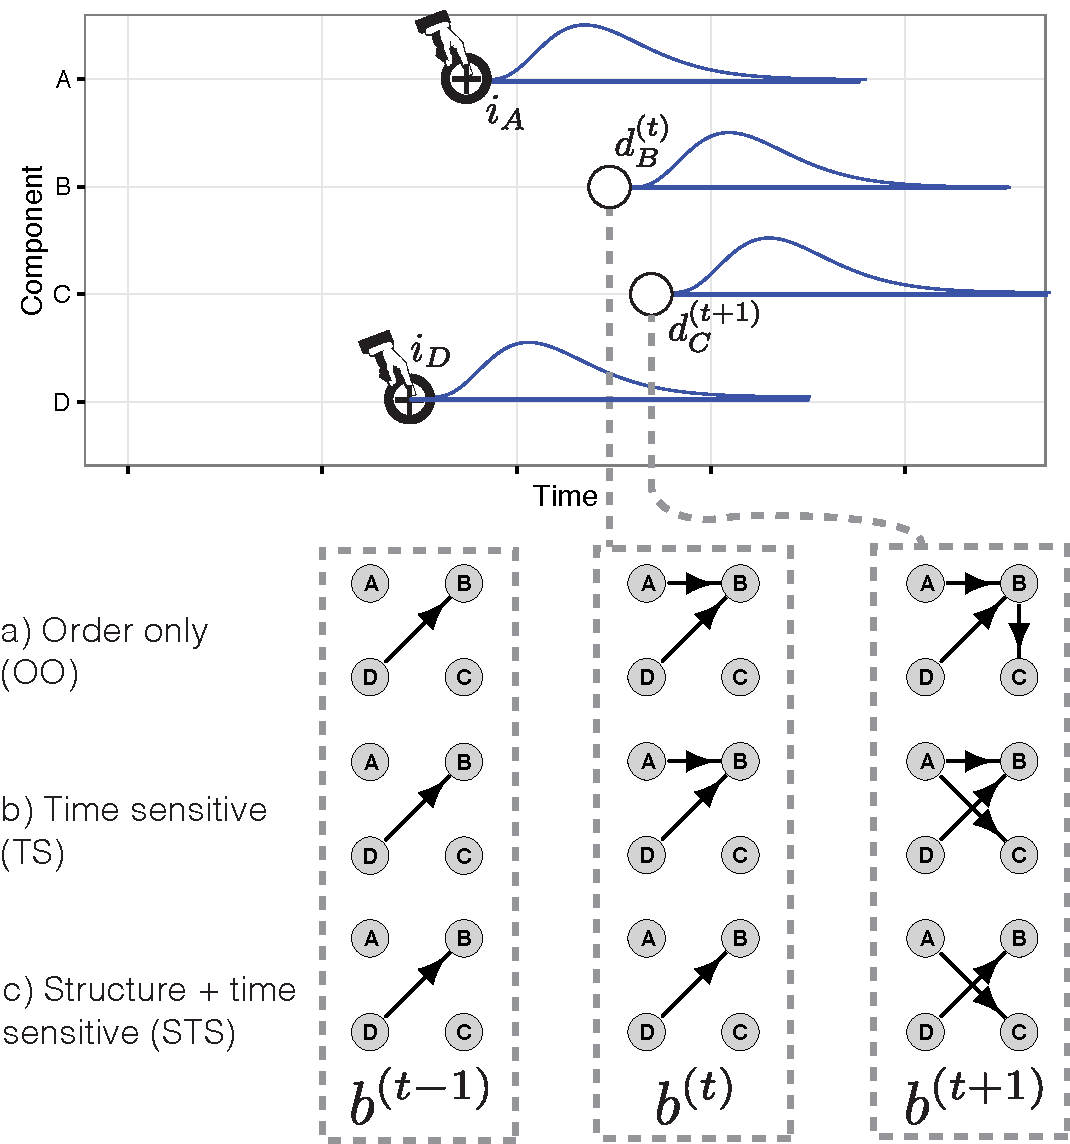
\includegraphics[width = .9\columnwidth]{heuristic_example}
   \caption[Continuous Time Causal Learning Heuristics]{An example in which the proposed heuristics make different model construction decisions.  $b^{(i-1)}$ is the learners belief at the start of the period depicted in the timeline plot.  After observing $d_B^{i}$ the models update $b^{(i-1)}$ to form $b^{(i)}$.  Then after observing $d_C^{i+1}$, they update again to form $b^{(i+1)}$.  Blue lines indicate the probability density for cause--effect delays starting from each event, used to determine the most likely cause of each event (TS), and whether it is sufficiently more likely than any existing causes (STS).}
   \label{fig:heuristic_example}
   \vspace{-0.6cm}
\end{figure}

\subsection{Model comparison procedure}

To compare the heuristics to participants' judgments, we simulated belief trajectories $\textbf{b}$s for all the heuristics based on the evidence generated by all participants, starting each trial with an unconnected model at $t=0$.  For TS and STS, we assumed knowledge of true $\mu$, $\alpha$ and $\ws$ as participants had been trained on these during the instructions. We predicted participants' judgments based on what the simulated belief trajectories looked like at judgment time. 
We then assessed their accuracy in the task (e.g. the proportion of connections marked correctly) and accordance rate (the proportion of connections marked the same as the matched participant's).  Additionally, we also compared participants to a \emph{Random} baseline that marked a new random causal structure on every judgment, and an Ideal learner that always selects the $\max P(M|\da_\tau;\ci_\tau, \ww)$ according to the Bayesian inference model.     

\subsection{Modeling results}

The results of these simulations are reported in Table~\ref{table:incremental_construction}.  Overall, \emph{STS} was the most closely concordant with participants but individually participants were almost evenly split between STS and OO, both for all judgments and restricted to the final judgments. %\footnote{We also tried variants of the models in which, after participants made a judgment, we updated $b^{(i-1)}$s of the models so that they matched the participants' current beliefs and updated them from there.  Doing this we get a larger number of participants best fit by STS (21) than OO (14), and none by Random or Ideal.}\srtodo{RM: The footnote could be deleted, I think.}%\ntodo{Dave says: why  not use as main analysis + need to explain why a footnote.\\I say: I don't mind, IMO the footnoted analysis shows a result that is better for distinguishing \emph{between} the heuristics because it zooms in on adaptations to what participants had actually already marked, but its worse for distinguishing \emph{whether} participants used the heuristics at all (because it boosts the fit of all of them relative to the Bayesian model so is an unfair test).  Tobi could you arbitrate perhaps?}
Participants accuracy ($0.65\pm0.19$) was closest to that of the simplest heuristic OO.  Mean participant accuracy by trial was correlated with that of all three heuristics $r_{\mathrm{OO}}=.83, r_{\mathrm{TS}}=0.92, r_{\mathrm{STS}}=0.61$, but negatively correlated with Ideal judgments $r_{\mathrm{Ideal}}=-.45$.

\begin{table}[ht]
\centering
\caption{Model comparison}
\vspace{-0.2cm}
\label{table:incremental_construction}
\footnotesize{
\begin{tabularx}{\columnwidth}{lXXXXXX}
\toprule
Model & \multicolumn{2}{l}{Accuracy (\%)}  & \multicolumn{2}{l}{Accordance (\%)}  & \multicolumn{2}{l}{N best (/40)}  \\ 
 & All & Final & All & Final & All & Final\\
\midrule
Random & 25.0 & 25.0 & 25.0 & 25.0 & 0 & 0 \\
OO & 66.2 & 64.7 & 67.2 & 64.9 & 16 & 17 \\ 
  TS & 79.7 & 78.9 & 67.3 & 65.5 &  4 &  5 \\ 
  STS & 87.9 & 90.9 & 69.3 & 69.2 & 15 & 13 \\ 
  Ideal & 91.0 & 95.3 & 66.1 & 68.9 &  5 &  5 \\
  % \hline
  % OO & 64.7 & 64.9 & 72.5 & 71.7 & 15 & 14 \\ 
  % TS & 75.5 & 75.6 & 73.0 & 73.4 &  5 &  5 \\ 
  % STS & 79.8 & 82.6 & 75.9 & 78.3 & 18 & 21 \\ 
  % Ideal & 91.0 & 95.3 & 66.1 & 68.9 &  2 &  0 \\ 
  \bottomrule
\end{tabularx}}
\footnotesize{\emph{Note:} ``N Best'' = the highest according model for each participant.}\raggedright
\vspace{-0.6cm}
\end{table}

\section{General Discussion}

In our experiment, people used interventions to learn about the causal structure of devices whose dynamics unfolded in continuous time.  As we predicted, cyclic structures were harder to learn than acyclic ones even though this was not reflected in the evidence available for an ideal learner, suggesting that the evidence produced by cyclic devices, involving many activations and potential causal paths, was harder for human learners to process.  We found that the observed determinants of successful learning -- equal spacing of interventions in time and a preference to intervene on root variables --- made structure inference easier for a heuristic and bounded learning system \citep{griffiths2015rational}.

In light of this, we considered several heuristic learning models. Participants' judgments were best explained by assuming that they added connections to a single evolving candidate hypothesis as they observed events. Some subjects appeared to rely on a simple order heuristic (OO) whereas others displayed sensitivity to the delays between events (TS) and whether events were predicted by existing structure beliefs (STS).  Participants rarely removed connections during the trials. Given longer to learn, however, it seems likely that they would also sometimes prune connections from their models --- e.g., when events predicted by their current model repeatedly fail to occur.  In general, positive testing of one's current hypothesis is an effective way for learners that are limited to a single global hypothesis to test its predictions against reality and tune, refine, or or even abandon it, if necessary. 

In sum, rather than grappling with an unmanageable space of possible structures and causal paths, participants seem to naturally follow Yogi Berra's advice: ``You don't have to swing hard [to hit a home run]. If you got the timing, it'll go.''
%\ttodo{not sure whether this last quote quite works (we can still drop it in the final version of course)}



\bibliographystyle{apacite}

\setlength{\bibleftmargin}{.125in}
\setlength{\bibindent}{-\bibleftmargin}

\def\thebibliography#1{\section*{References}
\scriptsize
 \list
 {[\arabic{enumi}]}{\leftmargin \parindent
   \itemindent -\parindent
   \itemsep 0ex plus 1pt
   \parsep 0.1ex plus 1pt minus 1pt
   \usecounter{enumi}}
   \def\newblock{\hskip .11em plus .33em minus .07em}
   \sloppy\clubpenalty4000\widowpenalty4000
   \sfcode`\.=1000\relax}

\bibliography{refs}

\end{document}
